\section{Experimental Settings}
\label{sec:experimental-settings}

In this section, we go through the experiments performed on our pipeline. We describe the parameter values and data used in the testing of each subproblem. Then, we present the results and briefly discuss them.

The implementation and the code used to generate each tested scenario are public and available in the following \href{https://github.com/aapolaakkio/thesis}{GitHub repository}.

\subsection{Data}

The data used to test the pipeline is synthetic, meaning it is randomly generated. We sample a per-graph scenario using a fixed graph id as the random-number-generator seed to ensure reproducibility. Each driver $k$ is assigned a shift start time $S_k\sim U(0, 60)$ and shift end time $H_k\sim U(240, 600)$, which together form the driver's shift window $[S_k, H_k]$, with both ends drawn from a uniform distribution. Each customer $i$ is drawn a wanted pickup time $U_i\sim U(0, 600)$ and a ride duration $R_i\sim U(5, 30)$. A delay cap $E_{\max}=15$ bounds how late a pickup can occur relative to the customer's wanted pickup time. Minimum break length $B_{\min}=10$ and maximum break length $B_{\max}=60$ are used to ensure some time between rides, simulating needing to move to a different location for the next pickup. We set the customer pickup delay and driver idle-time multipliers to $D=1$ and $I=1$. We charge a penalty $P=300$ for every customer that ends up unassigned.

We configure the bipartite graphs to have 3-6 edges for each customer, meaning 3-6 preferences per customer. We also allow at most 5 matched drivers for each customer. For drivers, we do not cap the number of matched customers, so theoretically all customers can be assigned to a single driver. In addition, we set the time granularity $\Delta t=1$, meaning scheduling is done at one-minute precision; we limit the resolution to at most 5 rounds, and each Gurobi run to at most 30 seconds.

We run 18 scenarios and one reference scenario. The number of customers was set as $N\in\{6000,7000,8000\}$ and number of drivers as $K\in\{100,110,120,130,140,150\}$. We run a scenario for every customer and driver count pair $N \times K$. We also run one additional reference with $N=1000$ and $K=200$ to test the pipeline's sensitivity.

\subsection{Matching results}

The first subproblem is finding the matching via maximum flow computation. For this subproblem, we record the maximum flow computed by the Ford–Fulkerson algorithm (max-flow), the time to compute the maximum flow and the matching ($t_{\text{FF}}$), the average customers per driver (cust./drv.) and average drivers per customer (drv./cust.). The results are presented in Table~\ref{tab:matching}.

\begin{table}[H]
\centering
\caption{Matching results}
\label{tab:matching}
\begin{tabular}{rrrrrr}
\toprule
$N$ & $K$ & max-flow & $t_{\text{FF}}$ (s) & cust./drv. & drv./cust. \\
\midrule
1000 & 200 & 4280 & 1.8  & 21.4 & 4.28 \\
6000 & 100 & 25469 & 65.4  & 254.7 & 4.24 \\
6000 & 110 & 25470 & 62.6  & 231.5 & 4.25 \\
6000 & 120 & 25511 & 62.4  & 212.6 & 4.25 \\
6000 & 130 & 25581 & 63.9  & 196.8 & 4.26 \\
6000 & 140 & 25516 & 64.9  & 182.3 & 4.25 \\
6000 & 150 & 25627 & 64.3  & 170.8 & 4.27 \\
7000 & 100 & 29805 & 85.7  & 298.1 & 4.26 \\
7000 & 110 & 29887 & 87.6  & 271.7 & 4.27 \\
7000 & 120 & 29644 & 85.6  & 247.0 & 4.23 \\
7000 & 130 & 29884 & 89.1  & 229.9 & 4.27 \\
7000 & 140 & 29759 & 87.1  & 212.6 & 4.25 \\
7000 & 150 & 29734 & 87.5  & 198.2 & 4.25 \\
8000 & 100 & 33933 & 113.3  & 339.3 & 4.24 \\
8000 & 110 & 34079 & 120.0  & 309.8 & 4.26 \\
8000 & 120 & 33963 & 113.4  & 283.0 & 4.25 \\
8000 & 130 & 34025 & 115.1  & 261.7 & 4.25 \\
8000 & 140 & 34011 & 121.0  & 242.9 & 4.25 \\
8000 & 150 & 34056 & 120.4  & 227.0 & 4.26 \\
\bottomrule
\end{tabular}
\end{table}

We observe that the maximum flow steadily increases as both the number of customers and the number of drivers increases. Increments in the number of customers cause a larger increase in the maximum flow than increments in the number of drivers. We also observe that the time to calculate the matching grows superlinearly with the number of customers, from an average of 64 seconds at $N = 6000$ to 117 seconds at $N = 8000$, and decreases slightly with the number of drivers.

The averages, however, behave a little differently. The average customers per driver increases as the number of customers increases but decreases as the number of drivers increases. This is logical, as drivers can match to a customer as long as there is an edge between them. Since drivers have no limit to the number of matched customers, only the number of edges generated between vertices limits the average. 

On the other hand, drivers per customer is almost the same across scenarios, averaging around $4.25$. This naturally happens because of the cap of 5 drivers per customer, and since there are always 3-6 edges per customer vertex, customers are matched to an average of $\frac{3+4+5+5}{4}=4.25$ drivers.

\subsection{Scheduling results}

The second subproblem is the per-driver scheduling. From this subproblem, we record the structure of the delivered schedule, i.e. the number of assigned (assig.) and unassigned customers (unassig.), the number of drivers that serve at least one customer (drv.\ used), the maximum (max load) and average number of customers per driver (avg load), the total pickup delay (delay) and idle time in minutes (idle), and the runtime of the first scheduling pass in seconds  ($t_{\text{sched}}$). Table~\ref{tab:scheduling} presents the results, and Figure~\ref{fig:sched-runtime} plots the runtime.

\begin{table}[H]
\centering
\caption{Scheduling results}
\label{tab:scheduling}
\small
\begin{tabular}{rrrrrrrrrr}
\toprule
$N$ & $K$ & assig. & unassig. & drv.\ used & max load & avg load & delay & idle & $t_{\text{sched}}$ \\
\midrule
1000 & 200 & 674 & 326 & 166 & 13 & 4.1 & 1642 & 64099 & 1.3 \\
6000 & 100 & 1789 & 4211 & 100 & 29 & 17.9 & 6914 & 18556 & 7.5 \\
6000 & 110 & 1818 & 4182 & 110 & 29 & 16.5 & 7039 & 19036 & 5.3 \\
6000 & 120 & 2069 & 3931 & 120 & 27 & 17.2 & 8408 & 21742 & 5.6 \\
6000 & 130 & 2202 & 3798 & 130 & 29 & 16.9 & 8430 & 23199 & 5.8 \\
6000 & 140 & 2290 & 3710 & 140 & 26 & 16.4 & 8801 & 24204 & 5.4 \\
6000 & 150 & 2442 & 3558 & 150 & 28 & 16.3 & 9159 & 26167 & 4.8 \\
7000 & 100 & 1835 & 5165 & 100 & 28 & 18.4 & 6960 & 19039 & 8.6 \\
7000 & 110 & 1935 & 5065 & 110 & 27 & 17.6 & 7803 & 20008 & 7.3 \\
7000 & 120 & 2165 & 4835 & 120 & 28 & 18.0 & 8568 & 22510 & 7.3 \\
7000 & 130 & 2371 & 4629 & 130 & 27 & 18.2 & 8759 & 24870 & 7.6 \\
7000 & 140 & 2524 & 4476 & 140 & 28 & 18.0 & 9180 & 26661 & 7.8 \\
7000 & 150 & 2675 & 4325 & 150 & 27 & 17.8 & 9804 & 28126 & 6.8 \\
8000 & 100 & 1877 & 6123 & 100 & 30 & 18.8 & 7597 & 19358 & 11.1 \\
8000 & 110 & 2087 & 5913 & 110 & 29 & 19.0 & 7872 & 21636 & 10.1 \\
8000 & 120 & 2219 & 5781 & 120 & 29 & 18.5 & 8276 & 23051 & 9.1 \\
8000 & 130 & 2380 & 5620 & 130 & 29 & 18.3 & 9181 & 24851 & 10.4 \\
8000 & 140 & 2490 & 5510 & 140 & 28 & 17.8 & 9562 & 26030 & 10.7 \\
8000 & 150 & 2758 & 5242 & 150 & 28 & 18.4 & 10865 & 28932 & 10.7 \\
\bottomrule
\end{tabular}
\end{table}

In every scenario, the number of served customers is limited by the driver capacity, not by the matching done in the previous subproblem. A driver's shift is on average about 390 minutes long, and a served ride takes on average $17.5 + B_{\min} = 27.5$ minutes, so a driver can serve roughly 14--26 customers depending on ride lengths. The observed maximum loads of 26--30 sit at the top of this range. Consequently, the number of assigned customers grows almost linearly with the number of drivers, by roughly 13 customers per added driver, while thousands of customers remain unassigned. Increasing the number of customers at a fixed driver count increases the assigned count only slightly. More customers give each driver more short rides to choose from, allowing denser packing of their shifts. Because every unassigned customer costs a penalty of $P = 300$, the unassigned term dominates the objective; for example, for $N = 6000$ and $K = 100$, the penalty term accounts for about 98\,\% of the final objective value.

The scheduling runtime grows superlinearly in the number of customers, from an average of 5.7 seconds at $N = 6000$ to 10.4 seconds at $N = 8000$, and shows no clear trend in the number of drivers (Figure~\ref{fig:sched-runtime}). This is expected, as more customers increase the size of each per-driver ILP, whereas adding a driver adds only one more independent ILP, optimized in parallel with the rest. All first-pass runtimes of the main scenarios stay between 4.8 and 11.1 seconds, and the reference scenario takes only 1.3 seconds, so the 30-second Gurobi time limit never constrains the solution.

\begin{figure}[H]
  \centering
  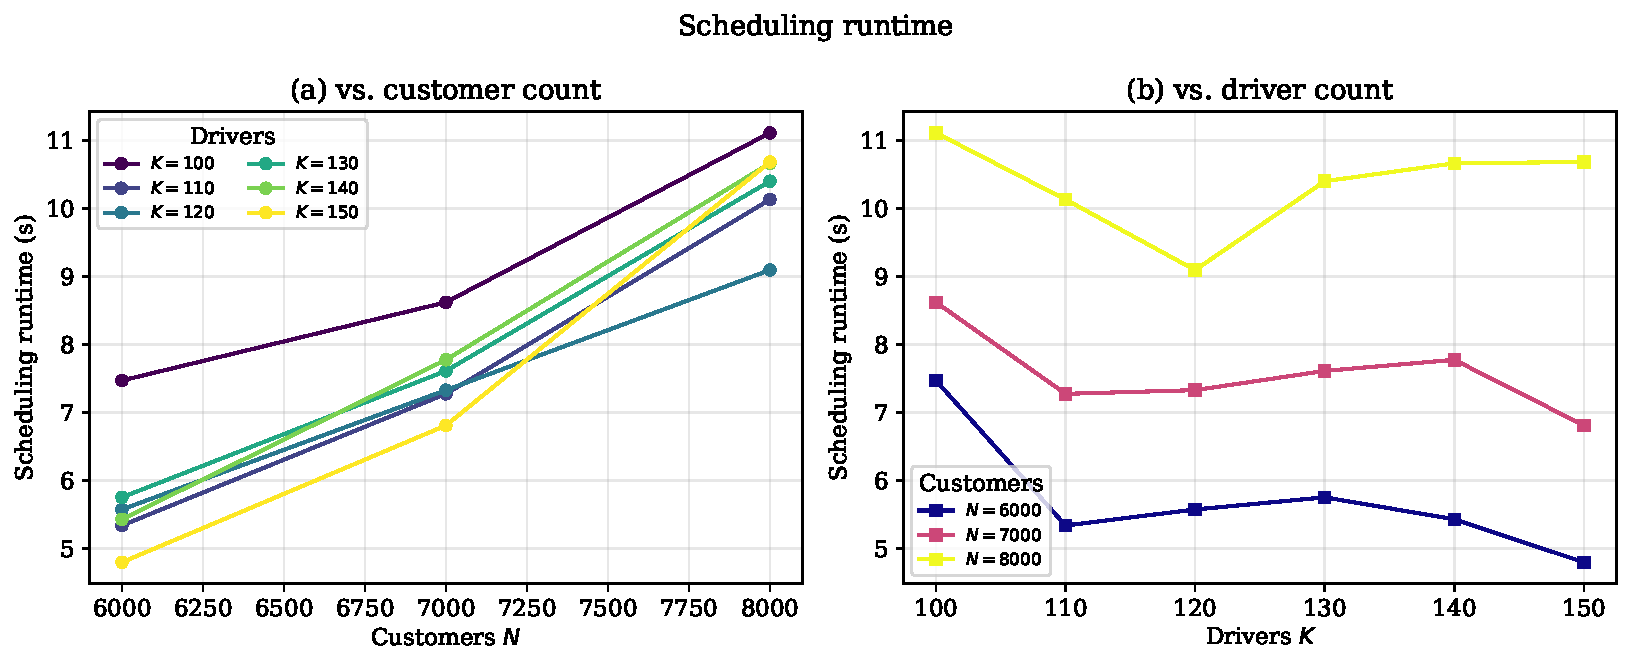
\includegraphics[width=\textwidth]{figures/results_scheduling_runtime.pdf}
  \caption{The runtime of the initial scheduling with respect to the number of customers and drivers}
  \label{fig:sched-runtime}
\end{figure}

The reference scenario with $N = 1000$ and $K = 200$ behaves differently. It is heavily over-provisioned, as only 166 of the 200 drivers serve any customers, and the average load is 4.1. Still, 326 customers remain unassigned. These customers likely cannot be served at all since a customer whose wanted pickup time falls late in the day fits inside the shift of only a small fraction of the drivers, and with on average 4.3 matched drivers per customer it is likely that none of them has a feasible start slot within the delay cap $E_{\max}$. Thus, the unassigned customers might not be a consequence of there being too few drivers. Instead this illustrates the possible effect of too strict preferences. With only one or two driver preferences, the risk of all preferred drivers not having a suitable ride slot becomes high.

\subsection{Conflict resolution results}

The last subproblem is the conflict resolution. From this subproblem, we record the objective value after the greedy assignment (initial) and after the iterated conflict resolution (final), the relative improvement between the two, the driver ordering that produced the best final objective, and the conflict resolution runtime $t_{\text{res}}$ in seconds. Table~\ref{tab:resolution} presents the results; Figure~\ref{fig:resolution-runtime} plots the runtime, Figure~\ref{fig:resolution-boxplot} compares the five driver orderings, and Figure~\ref{fig:objective-by-phase} shows the objective before and after the conflict resolution for every scenario.

\begin{table}[H]
\centering
\caption{Conflict resolution results}
\label{tab:resolution}
\small
\begin{tabular}{rrrrrlr}
\toprule
$N$ & $K$ & obj.\ initial & obj.\ final & improv.\ (\%) & strategy & $t_{\text{res}}$ \\
\midrule
1000 & 200 & 147704 & 163541 & -10.7 & load $\downarrow$ & 2.6 \\
6000 & 100 & 1464530 & 1288770 & +12.0 & load $\downarrow$ & 104.8 \\
6000 & 110 & 1454909 & 1280675 & +12.0 & index & 69.5 \\
6000 & 120 & 1408722 & 1209450 & +14.1 & load $\uparrow$ & 80.0 \\
6000 & 130 & 1383364 & 1171029 & +15.3 & index & 77.3 \\
6000 & 140 & 1365300 & 1146005 & +16.1 & confl. $\downarrow$ & 70.7 \\
6000 & 150 & 1329482 & 1102726 & +17.1 & confl. $\uparrow$ & 65.1 \\
7000 & 100 & 1757767 & 1575499 & +10.4 & index & 148.2 \\
7000 & 110 & 1742669 & 1547311 & +11.2 & confl. $\uparrow$ & 124.9 \\
7000 & 120 & 1681674 & 1481577 & +11.9 & confl. $\uparrow$ & 121.2 \\
7000 & 130 & 1647710 & 1422329 & +13.7 & confl. $\uparrow$ & 118.3 \\
7000 & 140 & 1624434 & 1378640 & +15.1 & confl. $\downarrow$ & 108.1 \\
7000 & 150 & 1596562 & 1335430 & +16.4 & confl. $\downarrow$ & 90.9 \\
8000 & 100 & 2047837 & 1863854 & +9.0 & load $\downarrow$ & 193.5 \\
8000 & 110 & 2009737 & 1803408 & +10.3 & load $\uparrow$ & 188.3 \\
8000 & 120 & 1980076 & 1765628 & +10.8 & confl. $\downarrow$ & 163.5 \\
8000 & 130 & 1950465 & 1720033 & +11.8 & confl. $\uparrow$ & 179.4 \\
8000 & 140 & 1926380 & 1688592 & +12.3 & load $\downarrow$ & 164.1 \\
8000 & 150 & 1883256 & 1612397 & +14.4 & confl. $\downarrow$ & 147.1 \\
\bottomrule
\end{tabular}
\end{table}

For all but the reference scenario, the iterated conflict resolution improves the objective by 9--17\,\%. The improvement grows with the number of drivers at every customer count, for example from 12.0\,\% at $K = 100$ to 17.1\,\% at $K = 150$ for $N = 6000$. This is expected as the conflict resolution improves the objective mainly by assigning previously unserved customers to drivers with spare capacity, each of which saves the penalty $P$, and a larger driver fleet has more spare capacity after the greedy pass. At a fixed number of drivers, the relative improvement decreases as the customer count grows, since the absolute gain stays similar while the objective itself grows with the number of unserved customers.

The resolution runtime grows superlinearly with the number of customers, from an average of 78 seconds at $N = 6000$ to 173 seconds at $N = 8000$, and decreases with the number of drivers (Figure~\ref{fig:resolution-runtime}), and it is roughly 15 times the first-pass runtime, as each of the five driver orderings reruns per-driver ILPs over several rounds. The runtime stays below 200 seconds in all scenarios.

\begin{figure}[H]
  \centering
  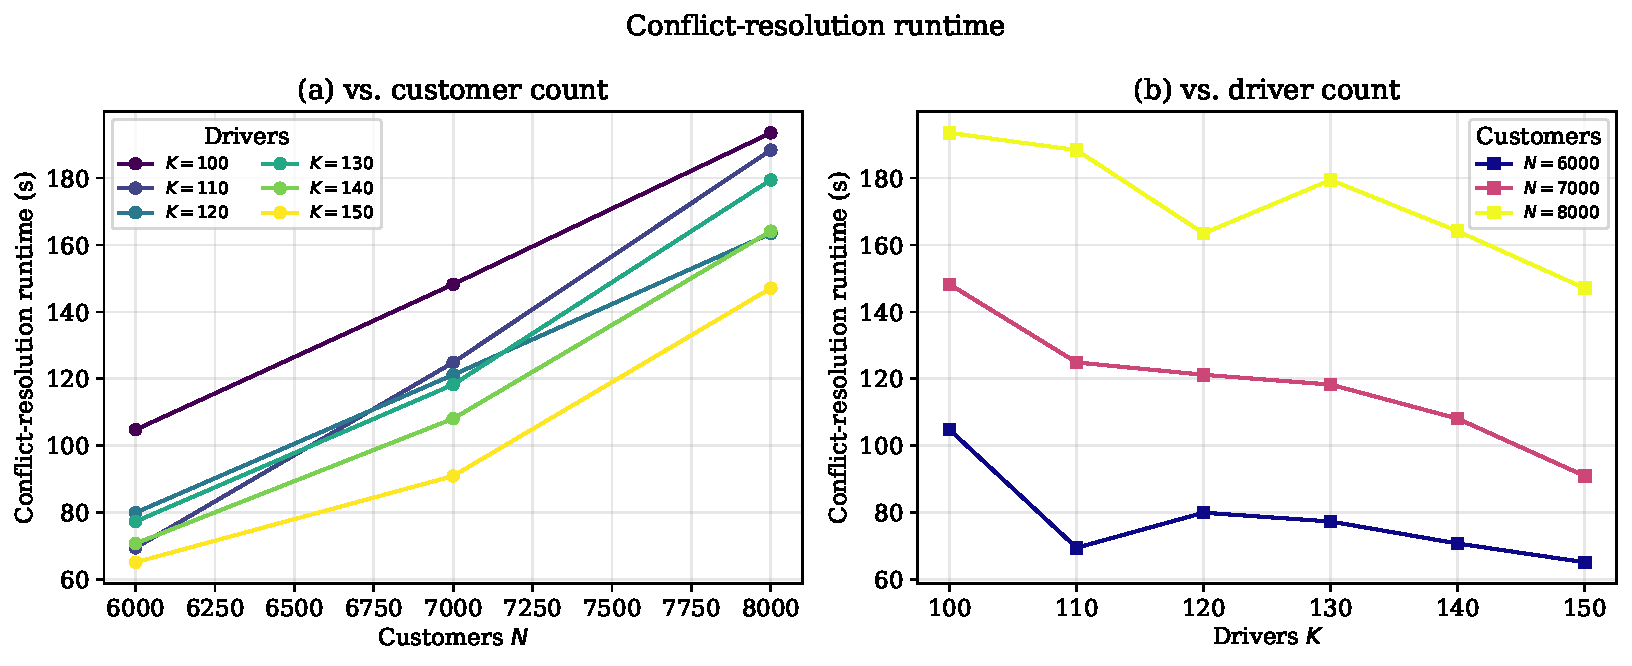
\includegraphics[width=\textwidth]{figures/results_resolution_runtime.pdf}
  \caption{The runtime of the conflict resolution with respect to the number of customers and drivers}
  \label{fig:resolution-runtime}
\end{figure}

Figure~\ref{fig:resolution-boxplot} shows that driver ordering matters little on average. The median excess over the per-scenario best ordering is below 0.11\,\% for every strategy, and no single ordering outperforms consistently, as shown in the chosen-strategy column of Table~\ref{tab:resolution}. The ascending-conflicts ordering has the lowest median excess, while the plain index ordering has the largest spread.

\begin{figure}[H]
  \centering
  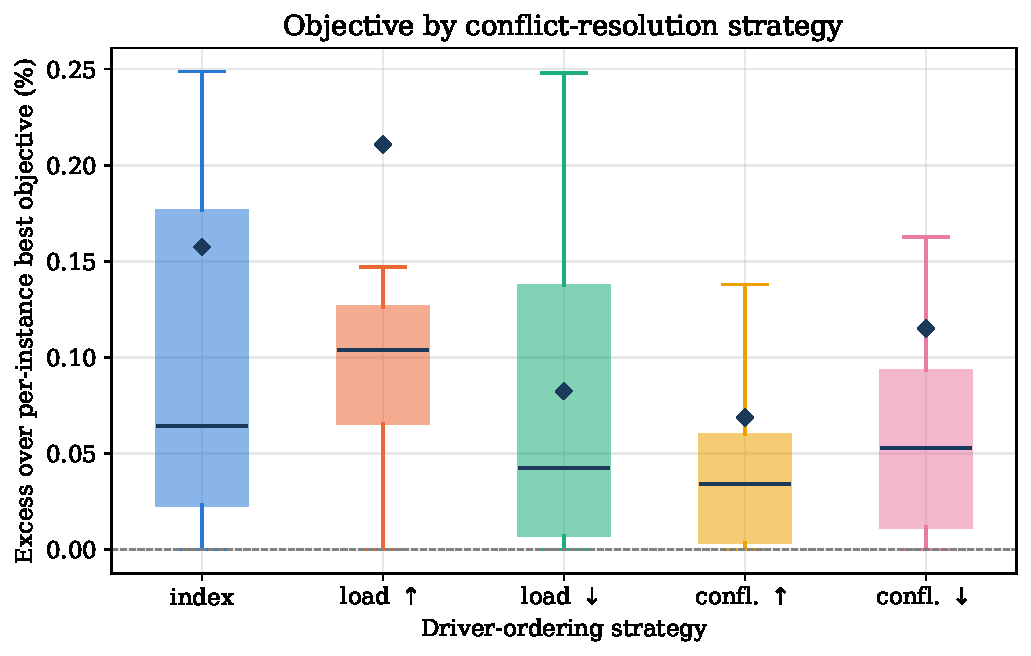
\includegraphics[width=\textwidth]{figures/results_resolution_boxplot.pdf}
  \caption{Excess of each driver-ordering strategy's objective over the per-scenario best. Outliers are omitted for readability.}
  \label{fig:resolution-boxplot}
\end{figure}

In the reference scenario, the resolution worsens the objective by 10.7\,\%. Each resolution is optimal for the driver itself but not necessarily
for the whole driver set. A driver assigned in the conflict resolution may drop a previously assigned customer back into the unserved pool, and in the over-provisioned reference scenario such swaps outweigh the few customers left to absorb them. The final result is the best of the five orderings; the initial greedy assignment is not kept as a candidate, so the pipeline does not fall back to it even when every ordering ends worse. Adding the greedy assignment as a sixth candidate would remove this failure mode.

\begin{figure}[H]
  \centering
  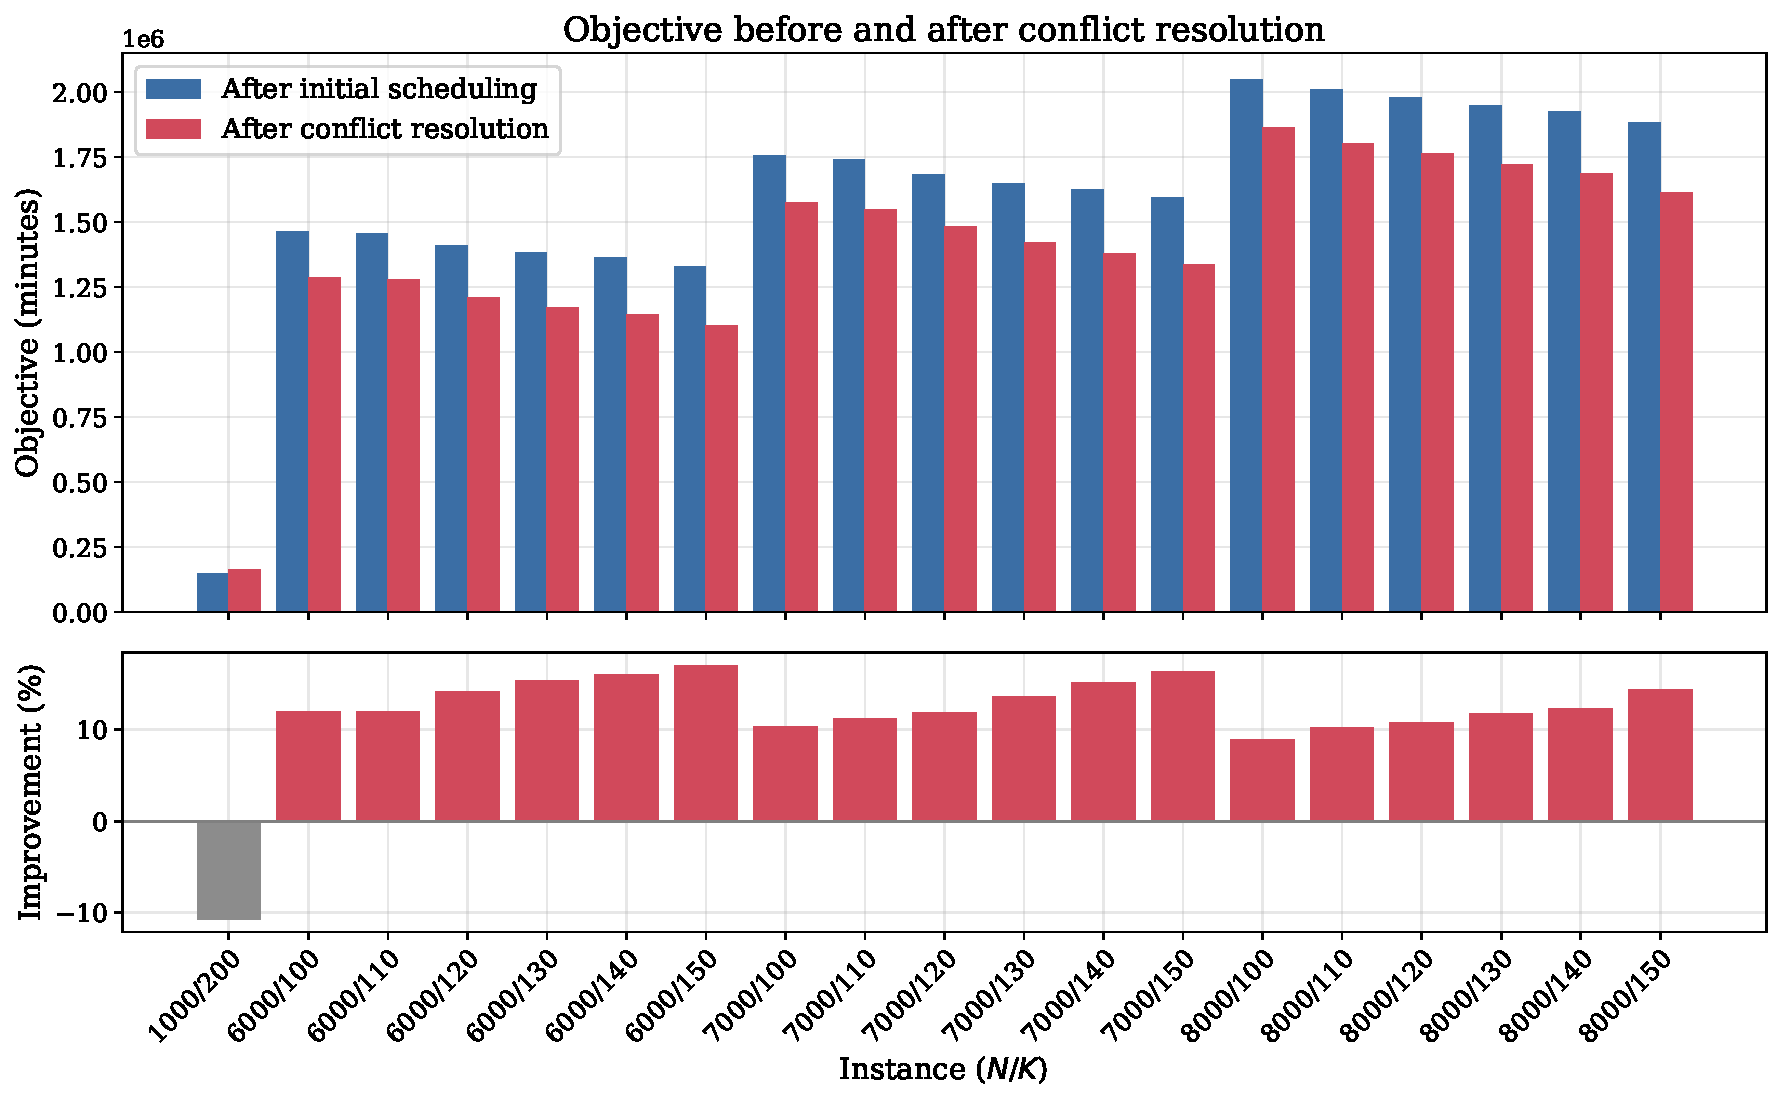
\includegraphics[width=\textwidth]{figures/results_objective_by_phase.pdf}
  \caption{Improvement of scheduling objective between the initial scheduling round and after resolving}
  \label{fig:objective-by-phase}
\end{figure}
